\section{Testfälle}
\subsection{Eindimensionale Testfälle}

Die Testfälle im eindimensionalen Raum setzen als Problemgebiet das
Intervall $[0,1]$ fest. Eine Transformation von diesem Intervall auf jedes 
andere zusammenhängende Intervall ist möglich.

Der erste eindimensionale Testfall stellt eine symmetrische Sinusfunktion
dar. Es wird eine halbe Periode genutzt. Um auch die Randbedingungen zu testen,
wird sie eine Einheit nach oben geschoben. \begin{equation}
f(x) = \sin(\pi x)+1
\end{equation}
\begin{figure}[h]
\begin{tikzpicture}
\begin{axis}[
xlabel=$x$,
ylabel={$f(x)$},
domain=0:1,
height=4cm,
width=0.6*\textwidth
]
% use TeX as calculator:
\addplot +[mark=none, samples=100,very thick,tud2d]{sin(pi*deg(x))+1};
\end{axis}
\end{tikzpicture}
\centering
\caption{Testfunktion 1 im Intervall [0,1]}
\label{fig:testfn1}
\end{figure}


\noindent
Der zweite Testfall stellt eine unsymmetrische Funktion dar. Es handelt sich um
die halbe Periode der Kosinusfunktion, welche um eine Einheit nach unten verschoben wurde.
\begin{equation}
f(x) = \cos(\pi x) -1
\end{equation}
\begin{figure}[h]
\begin{tikzpicture}
\begin{axis}[
xlabel=$x$,
ylabel={$f(x)$},
domain=0:1,
height=4cm,
width=0.6*\textwidth
]
\addplot +[mark=none,samples=100, very thick,tud2d]{cos(pi*deg(x))-1};
\end{axis}
\end{tikzpicture}
\centering
\caption{Testfunktion 2 im Intervall [0,1]}
\label{fig:testfn2}
\end{figure}

\clearpage
\subsection{Zweidimensionale Testfälle}

Auch die zweidimensionalen Testfälle legen als Problemgebiet das Intervall
$[0,1]\times[0,1]$ fest. Wie im Eindimensionalen kann dieses durch Transformation
in jedes andere zusammenhängende Intervall überführt werden.

Der erste zweidimensionale Testfall ist symmetrisch und testet alle
Randbedingungen.
\begin{equation}
f(x,y) = \sin(\pi x) \sin(\pi y) + 1
\end{equation}

\begin{figure}[h]
\centering
\begin{subfigure}[b]{.5\linewidth}
\centering
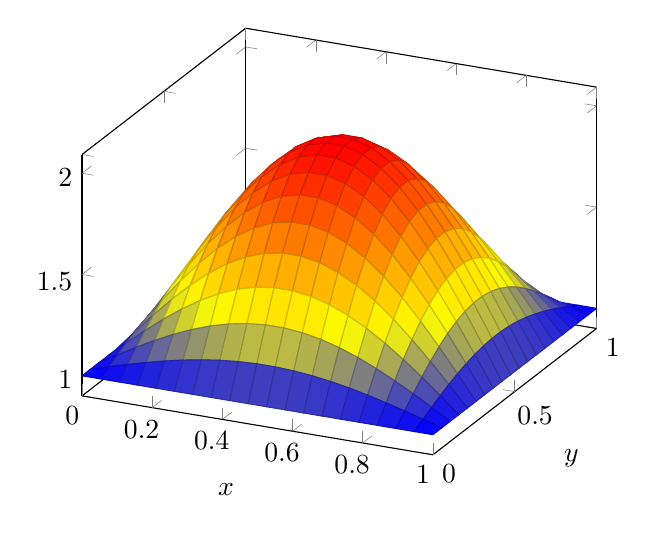
\begin{tikzpicture}
\begin{axis}[
xlabel=$x$,
ylabel=$y$,
%zlabel={$f(x,y) = \sin(\pi x) \sin(\pi y) + 1$},
domain=0:1,
height=7cm
]
\addplot3 +[surf, mark=none, samples=20]{sin(pi*deg(x))*sin(pi*deg(y))+1};
\end{axis}
\end{tikzpicture}
%\subcaption{Oberflächen}\label{fig:1a}
\end{subfigure}%
\begin{subfigure}[b]{.5\linewidth}
\centering
\begin{tikzpicture}
\begin{axis}[
view={0}{90},
xlabel=$x$,
ylabel=$y$,
zlabel={$f(x,y) = \sin(\frac{\pi}{2} x) \cos(\frac{\pi}{2} y)$},
domain=0:1,
height=7cm
]
\addplot3 +[contour prepared,very thick,mark=none, contour prepared format=matlab]
file {data/3_contour.txt};
\end{axis}
\end{tikzpicture}
%\subcaption{Another subfigure}\label{fig:1b}
\end{subfigure}
\caption{Testfunktion 3 im Intervall [0,1]$\times$[0,1]}\label{fig:tf3}
\end{figure}

\noindent
Die zweite zweidimensionale Testfunktion ist unsymmetrisch. Ihre Gleichung lautet:
\begin{equation}
f(x,y) = \sin(\frac{\pi}{2} x) \sin(\frac{\pi}{2} y)
\end{equation}
\begin{figure}[h]
\centering
\begin{subfigure}[b]{.5\linewidth}
\centering
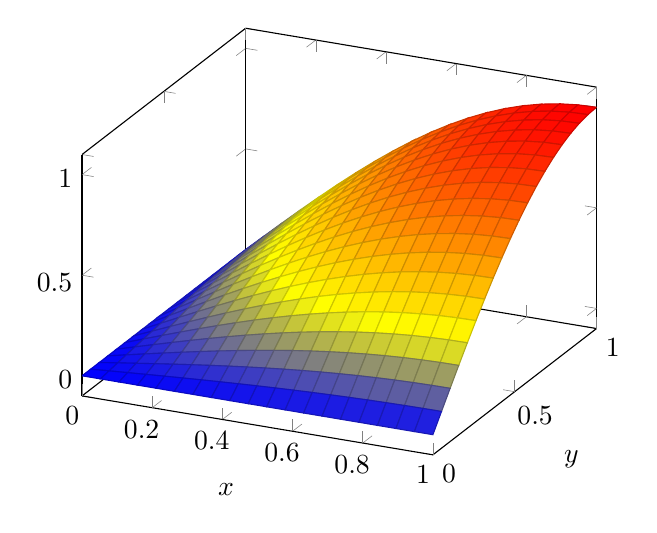
\begin{tikzpicture}
\begin{axis}[
%view={30+180}{30},
xlabel=$x$,
ylabel=$y$,
%zlabel={$f(x,y) = \sin(\frac{\pi}{2} x) \cos(\frac{\pi}{2} y)$},
domain=0:1,
height=7cm,
]
\addplot3 +[surf, mark=none, samples=20]{sin(pi/2*deg(x))*sin(pi/2*deg(y))};
\end{axis}
\end{tikzpicture}
%\subcaption{Oberflächen}\label{fig:1a}
\end{subfigure}%
\begin{subfigure}[b]{.5\linewidth}
\centering
\begin{tikzpicture}
\begin{axis}[
view={0}{90},
xlabel=$x$,
ylabel=$y$,
zlabel={$f(x,y) = \sin(\frac{\pi}{2} x) \sin(\frac{\pi}{2} y)$},
domain=0:1,
height=7cm
]
\addplot3 +[contour prepared,very thick,mark=none, contour prepared format=matlab]
file {data/4_contour.txt};
\end{axis}
\end{tikzpicture}
%\subcaption{Another subfigure}\label{fig:1b}
\end{subfigure}
\caption{Testfunktion 4 im Intervall [0,1]$\times$[0,1]}\label{fig:tf4}
\end{figure}

\clearpage
